\subsection{Галактики}
\term{Морфологическая классификация галактик}~--- система разделения галактик на группы по визуальным признакам, используемая в астрономии. Наиболее известной является классификация, разработанная Хабблом и дополненная другими учеными. 
	\begin{figure}[h!]
		\centering
		\vspace{-.9pc}
		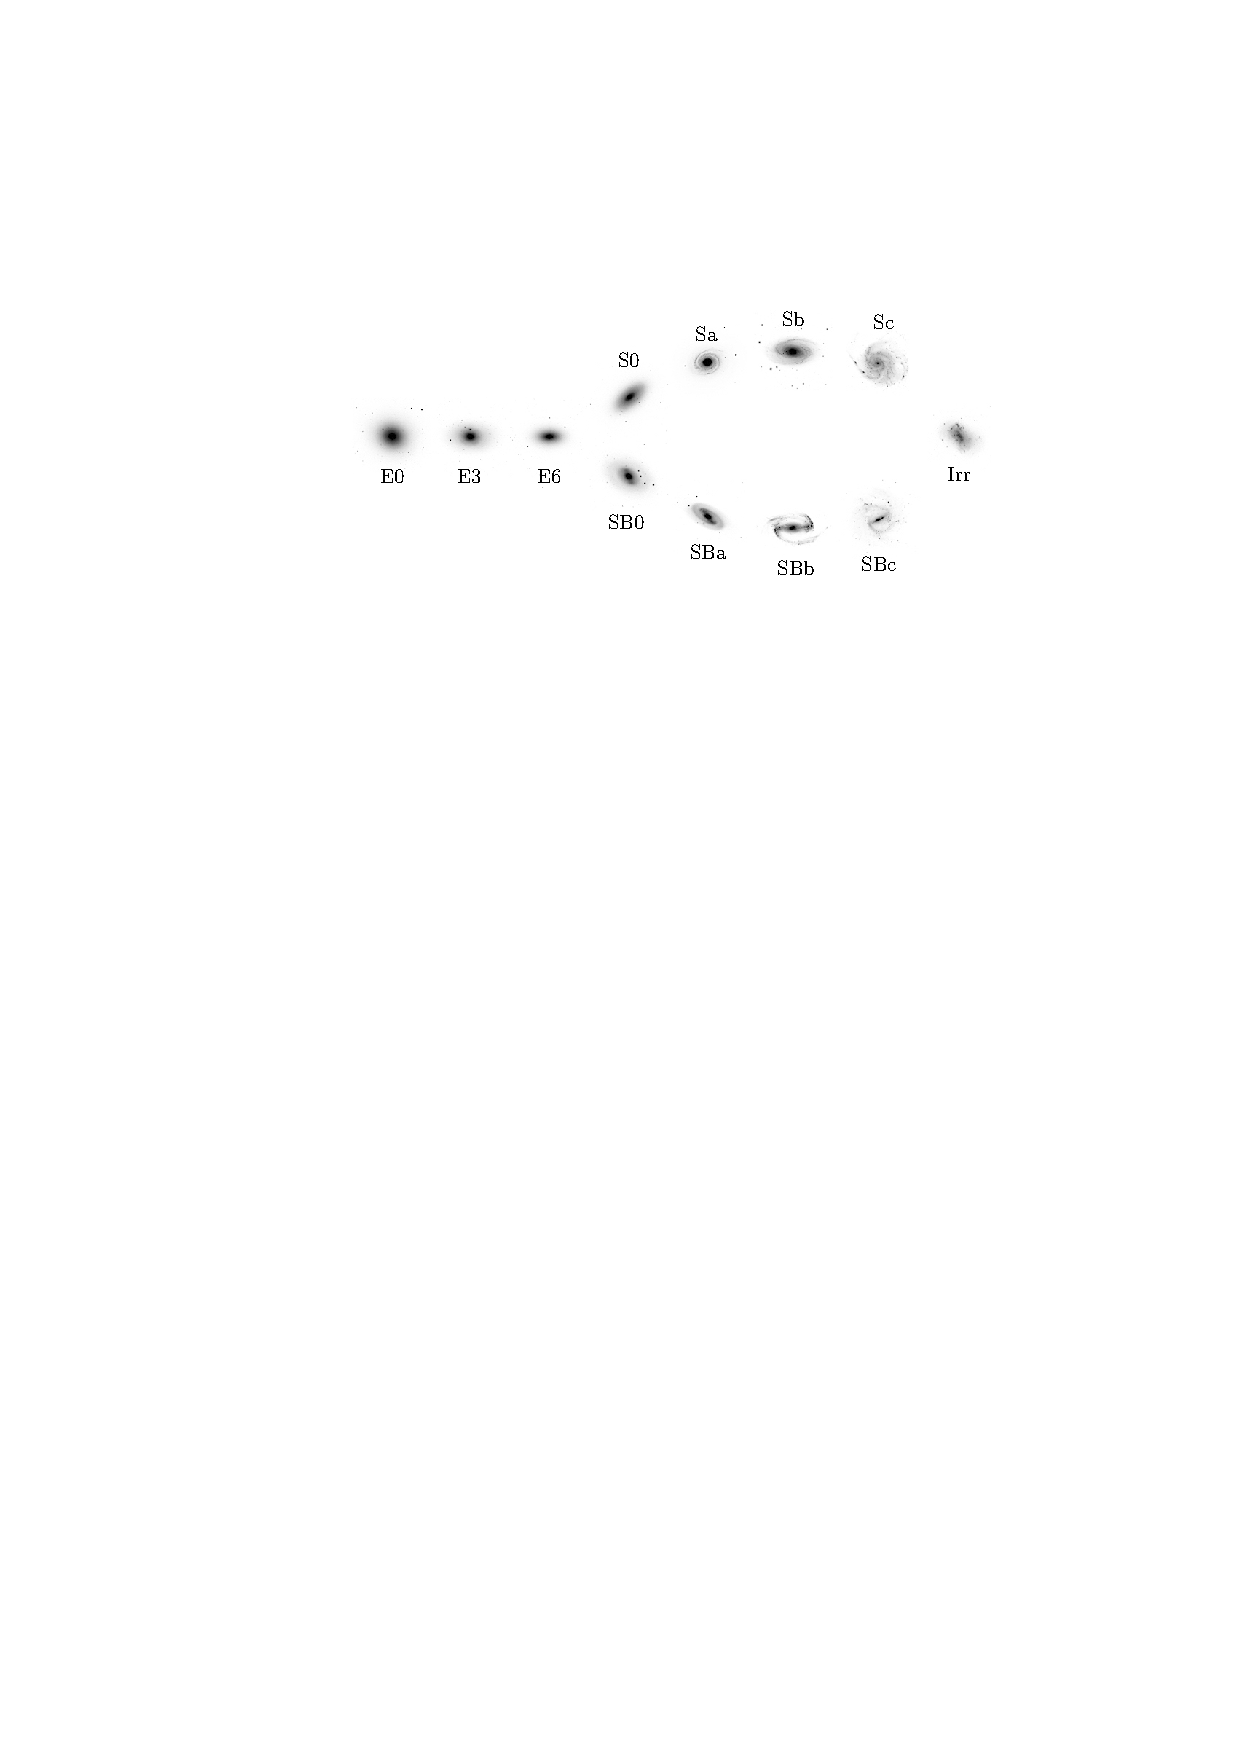
\includegraphics[width=0.65\tw]{hubble-fork.pdf}
		\caption{<<Вилка Хаббла>>}
	\end{figure}
	
Согласно данной классфикации галактики делятся на 4 типа:
\begin{enumerate}[itemsep=3pt, label={\arabic*.}, leftmargin=1pc]
	\item{\term{Эллиптические галактики} имеют гладкую эллиптическую форму без отличительных деталей с равномерным уменьшением яркости от центра к периферии. Обозначаются буквой E с индексом. Индекс можно рассчитать по формуле
		\begin{equation}
		i = 10 \times \left(1 - \frac{b}{a}\right),
		\end{equation}
		где $a$ и $b$~--- большая и малая полуоси видимого эллипса.}
	\item{\term{Спиральные галактики} состоят из уплощенного диска из звезд и газа, в центре которого находится сферическое уплотнение, называемое балджем, а также обширного сферического гало. Спиральные галактики обозначаются SB при наличии бара (перемычки между рукавами) или S при отсутствии бара. В зависимости от размеров ядра и балджа галактики делят на 3 группы: a, b и c. Для галактик Sa характерен большой балдж, для галактик Sc~--- маленький. Галактики Sb представляют собой нечто среднее между галактиками Sa и Sb.
	
	Светимость спиральных галактик $L$ связана с их максимальной скоростью вращения $v_\text{макс}$ \term{соотношением Талли-Фишера}:
	\begin{equation}
		L \propto v_\text{макс}^4.
	\end{equation}
	Абсолютная звёздная величина Млечного пути $M_\text{MW} \simeq -21^m$.}
	\item{\term{Неправильные или иррегулярные галактики}~--- галактика, лишенная как вращательной симметрии, так и значительного ядра. Обозначение: Irr.}
	\item{\term{Линзовидные галактики}~--- галактики, являющиеся переходными между спиральными и эллиптическими. Обозначения: S0, SB0.
	
	К линзовидным галактикам с абсолютной звёздной величиной около $-21^m$ применимо соотношение Фабер-Джексона:
	\begin{equation}
		L \propto v^4,
	\end{equation}
	где $v$~--- скорость вращения вещества.}
\end{enumerate}

